\section{Motor model}
\label{Sect:1}
This section must include motor rated parameters (as input data), key equations and description of direct and inverse flux maps, as well as MTPA profiles.

\subsection{Motor data}
This section is dedicated to illustrate the motor parameters and useful data.

\begin{table}[!h]
	\captionsetup{justification=justified}
	\caption{Motor data.}
	\label{tab:Motor_data}
	\centering
		\begin{tabular}{@{}lccc@{}} 
		\toprule
		\toprule
		\textbf{Symbol} & \textbf{Quantity} & \textbf{Unit}\\ 
		\midrule
		---		& --- 	& ---	\\
		---		& --- 	& ---	\\
		\bottomrule
		\end{tabular}
	\vspace{-10pt}
\end{table}


\subsection{Motor equations}
This subsection is dedicated to main motor equations.

\subsection{Flux maps and MTPA}
This subsection is dedicated to direct and inverse flux maps and also for MTPA profiles.


\par See https://en.wikibooks.org/wiki/LaTeX/Mathematics for more info.
\par See in eq. \eqref{eq:EltEq}.
\begin{equation}
	\begin{array}{ccc}
		v_{d} &=& -R_{s} i_{d} - \upomega_r \uplambda_{q} + \dfrac{1}{\upomega_b}\dfrac{d\uplambda_{d}}{dt} \\[15pt]
		v_{q} &=& -R_{s} i_{q} + \upomega_r \uplambda_{d} + \dfrac{1}{\upomega_b}\dfrac{d\uplambda_{q}}{dt}\\[15pt]
		\uptau_{rq0} \dfrac{d \uplambda_{rq}}{dt}&=& -\uplambda_{rq} - L_{rq} i_{q}
	\end{array}
	\label{eq:EltEq}
\end{equation}

\begin{equation}
v_{q}=R_s\cdot i_q
\label {Equ:2}
\end{equation}


\begin{equation}
A = 
		\begin{bmatrix}
			A_{1} & 0 & \dotsi & 0\\
			0 & A_{2} & \dotsi & 0\\
			\vdots & \vdots & \ddots & \vdots\\
			0 & 0 & \dotsi & A_{n}
		\end{bmatrix}
\end{equation}

\par Greek letters. I suggest the package upgreek to write upright Greek letters. For example $\upomega$ is from upgreek, while $\omega$ is the standard letter. Capital Greek letters are $\upOmega$.


\subsection{EXAMPLE LISTS}
\begin{enumerate}
	\item OBJ 1
	\item OBJ 2
	\item Method 3
\end{enumerate}

\begin{itemize}
	\item OBJ 1
	\item OBJ 2
\end{itemize}

\subsection{EXAMPLE TABLE}
\begin{table}[!h]
	\captionsetup{justification=justified}
	\caption{Table caption.}
	\label{tab:ExTab}
	\centering
		\begin{tabular}{@{}lccc@{}} \toprule
		\textbf{Parameter} & \textbf{Value} & \textbf{Parameter} & \textbf{Value} \\ \midrule
		$V_b$	& $120 \sqrt{2}$ V& $S_b$	& 15 kVA\\
		$L_f$   & 545 $\upmu$H & $C_f$ & 22 $\upmu$F\\
		$L_{fg}$& 120 $\upmu$H & $L_g$ & 270 $\upmu$H\\ 
		$L_{s}$& 0.1 pu & $R_s$ & 0.02 pu\\
		$H$& 4 s & $\uptau_e$ & 0.1 s\\
		$L_{rq}$& 0.71 pu & $\uptau_{rq0}$ & 0.23 s\\
		\bottomrule
		\end{tabular}
	\vspace{-10pt}
\end{table}

\subsection{EXAMPLE FIGURES}
\par EXAMPLE FIGURES. Figures can be in png, pdf, eps. svg and emf are not supported.
Figure parameters: In square brackets the positioning attributes t=top, b=bottom, h=here, p=newPage, !=force positioning.
\par Figure references: As it can be seen in Fig.~\ref{fig:SingleFigure}.
\par Single Figure.
\begin{figure}[t]
	\centering
	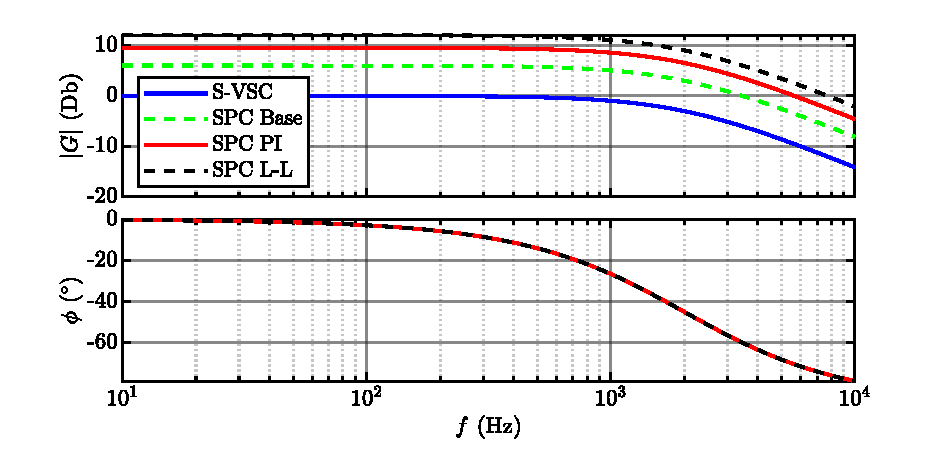
\includegraphics[width=\columnwidth]{Example01.pdf}
	\captionsetup{justification=justified}
	\caption{Caption line 1. \newline Caption Line 2.}
	\label{fig:SingleFigure}
\end{figure}

\par Subfigures.
\begin{figure*}[t]
	\centering
	\subfloat[]{
\includegraphics[width=0.5\textwidth]{ExFig.pdf}}
	\subfloat[]{
\includegraphics[width=0.5\textwidth]{ExFig.pdf}}
	\captionsetup{justification=justified}
	\caption{This is a subfloat with horizontal alignment. \newline Caption Line 2.}
	\label{fig:adjacentFigs}
	\vspace{-5mm}			%This reduces the vertical space after a figure.
\end{figure*}

\par This is an additional paragraph.

\begin{figure}[t] 
	\centering
	\subfloat[]{
\includegraphics[width=\columnwidth]{ExFig.pdf}}
	\vfil
	\subfloat[]{
\includegraphics[width=\columnwidth]{ExFig.pdf}}
	\captionsetup{justification=justified}
	\caption{Caption line 1. \newline Caption Line 2.}
	\label{fig:ColumnFigs}
	\vspace{-4.5mm}
\end{figure}